\documentclass[11pt]{article}
\usepackage[margin=1in]{geometry}
\usepackage[round]{natbib}
\usepackage{graphicx}
\usepackage{amsmath}
\usepackage{amssymb}
\usepackage{float}
\usepackage[parfill]{parskip} % new line between paragraphs, no indentation
\usepackage[colorlinks,pdfstartview=FitH,citecolor=blue]{hyperref}
\usepackage{xcolor}
\usepackage{xeCJK} % Enabling Chinese characters

% Header
\usepackage{fancyhdr}
\pagestyle{fancy}
\fancyhf{}%Clear all heads and foots
\setlength{\headheight}{40pt} %Eliminate the warning of "headheight is too samll"
\rhead{PM2.5 Modeling\\Jianzhao Bi\\\today}
\cfoot{\thepage}


\begin{document}

\setcounter{tocdepth}{1} % Set the depth of the TOC
\tableofcontents
\newpage 

% =================================

\section{AOD/PM2.5 measurements and visualization}

\paragraph{\citet{van2006estimating}}
\begin{itemize}
    \item \textbf{Not plotting annual mean PM2.5 with few daily coverage}: White areas indicate ocean or regions with AOD measurements on fewer than either 40\% of days for MODIS or 8\% of days for MISR.
    \item AQS and NAPS (Canada): Both networks collect continuous measurements primarily from tapered element oscillating microbalance (\textbf{TEOM}) instruments, which infer the collected PM2.5 mass from changes in the natural frequency of the oscillator. 
    \item \textbf{AERONET AOD uncertainty}:  AERONET measurements of AOD have an uncertainty of $\sim$0.01 -- 0.02 \citep{holben2001emerging}.
\end{itemize}

\paragraph{\citet{van2010global}}
\begin{itemize}
    \item Point measurements collected at monitoring sites are not necessarily representative of regional concentration, and regional variability is difficult to assess from point measurements alone. 
    \item When using CTM, relative humidity of PM2.5 measurements should be considered: We applied modeled relationship between aerosol mass and \textbf{relative humidity} for each aerosol type to calculate PM2.5 for relative humidity values that correspond to surface measurement standards. 
    \item The inconsistency between satellite and \textit{in situ} measurements: many factors contribute to the inconsistency, including differences between what satellite and \textit{in situ} measurements represent, that do not necessarily indicate errors in either measurement.
    \item Sampling errors in annual PM2.5: Sampling error of satellite-derived PM2.5 is larger in regions influenced by biomass burning, mineral dust, or persistent cloud because of a combination of large seasonal variability and nonrepresentative sampling. We applied the ratio of complete to coincident mean simulated PM2.5 to reduce uncertainty from sampling variability.
\end{itemize}

\paragraph{\citet{zimmerman2018machine}}
\begin{itemize}
    \item The variable importance of random forest from different models (e.g., daily models) can be visualized as box plots
    \begin{figure}[H]
        \centering
        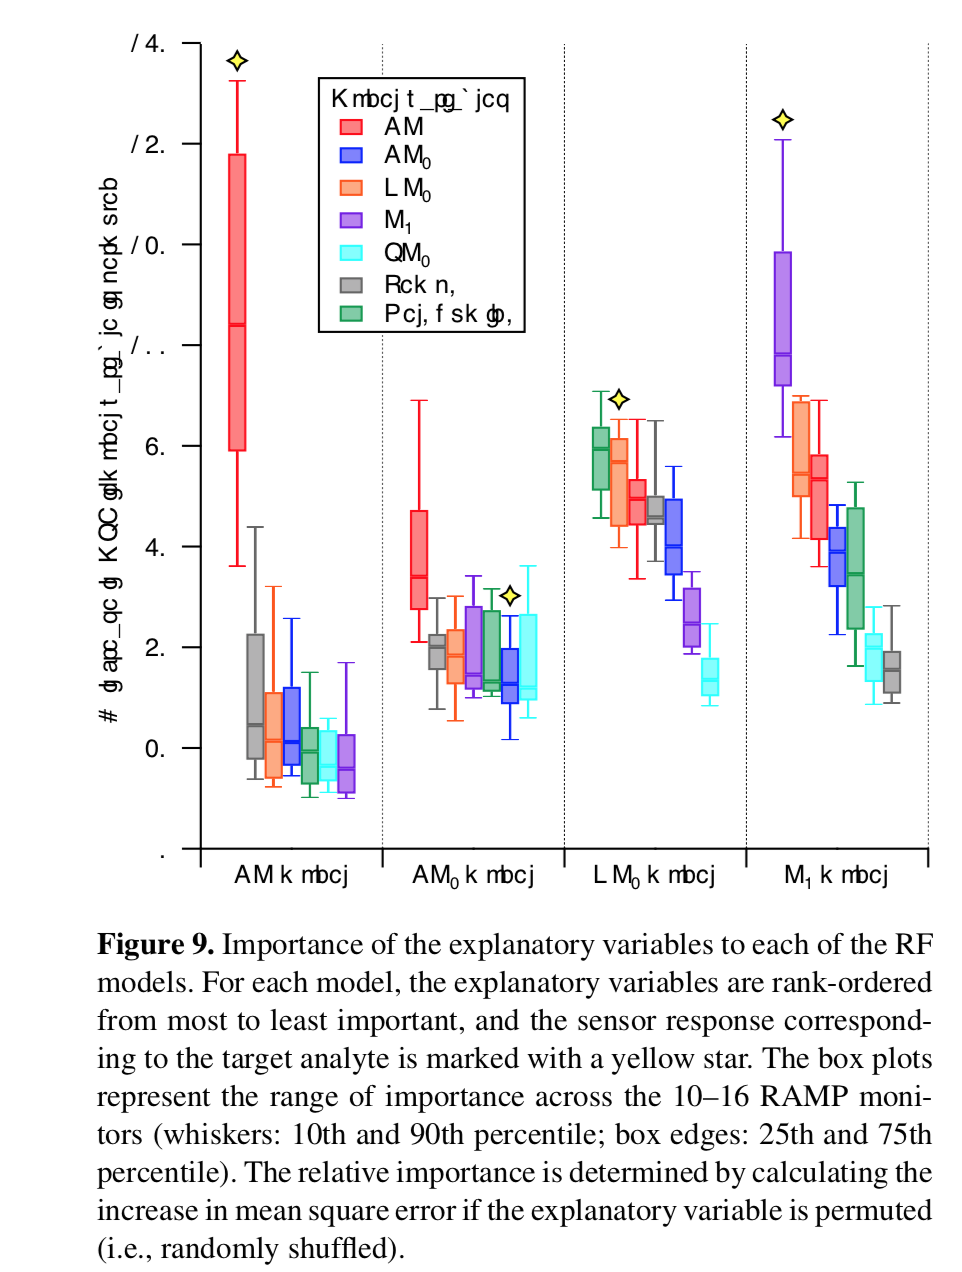
\includegraphics[width=0.5\textwidth]{img/rf_imp.png}
        \label{fig:rf_imp}
    \end{figure}
\end{itemize}

% =================================

\section{Factors affecting PM2.5 estimation from satellite AOD}

\paragraph{\citet{van2006estimating}}
\begin{itemize}
    \item Empirical relationships between remotely measured AOD and surface PM2.5 have been developed for the southeast United States using both MODIS and MISR. A common concern is the dependence upon several factors in addition to the AOD measurement, including the \textbf{aerosol vertical profile, aerosol type and atmospheric conditions}. 
    \item \textbf{Important factors} in PM2.5 estimation:  
        \begin{itemize}
            \item Spatially: The \textbf{relative vertical profile of aerosol extinction} is the dominant parameter in determining the spatial variation between AOD and PM2.5 over North America. 
            \item Temporally: Daily variation in \textbf{AOD} played the major role in accurately representing daily variation in remote-sensed PM2.5. 
        \end{itemize}
    \item Despite large AOD over and downwind of the Sahara, low PM2.5 concentrations ($< 5 \mu g/m^3$) result from strong vertical mixing and a large coarse aerosol fraction.
\end{itemize}

\paragraph{\citet{van2010global}}
\begin{itemize}
    \item The applicability of AOD to surface air quality depends on several factors, including the \textbf{vertical structure, composition, size distribution, and water content of atmospheric aerosol}.
    \item $PM2.5=\eta\times AOD$
    \begin{itemize}
        \item $\eta$ is a function of the factors that relates 24-hr dry aerosol mass to satellite observations of ambient AOD: aerosol size, aerosol type, diurnal variation, relative humidity, and the vertical structure of aerosol extinction \citep{van2006estimating}.
        \item Average values of $\eta$ are typically $20 - 130 \mu g/m^3$. High values of $\eta$ over regions with large dust concentrations \citep{prospero2002environmental} reflect, in part, the low hygroscopicity of dust. Values of $\eta$ are lower for hygroscopic aerosols, as their dry volume is significantly smaller than under ambient conditions.
        \item Western North America is characterized by low $\eta$, which provides additional insight into the poor AOD -- PM2.5 correlations associated with this region and in agreement with \citet{liu2007estimating}, who found that transported dust aloft affects the western North America AOD -- PM2.5 relationship. 
        \item Application of $\eta$ in deriving PM2.5 increased the spatial contrast relative to $\eta$ itself, which reflects ground-level aerosol sources in the east and aerosols aloft in the north and west.
    \end{itemize}
\end{itemize}

% =================================

\section{CTM AOD and PM2.5}

\paragraph{\citet{van2010global}}
\begin{itemize}
    \item Satellite/CTM-derived PM2.5 is better than CTM PM2.5:  Notably, this level of agreement with ground-based PM2.5 significantly better than that obtained using a global CTM (GEOS-Chem) without satellite data. 
\end{itemize}

% =================================

\section{AOD/PM2.5 distributions and sources}

\paragraph{\citet{van2006estimating}}
\begin{itemize}
    \item Elevated PM2.5 in \textbf{California} is associated with high emissions of aerosol precursors and topography that is exacerbated in winter by low mixing height, coupled with the thermodynamic tendency for ammonium nitrate to exist in aerosol phase at lower wintertime temperatures. 
    \item Southeastern PM2.5 concentrations in the US are driven largely by organics, emitted directly by fires and formed as secondary organic aerosol from biogenic hydrocarbons; processes which are most active during warm seasons \citep{malm2004spatial}.
    \item \textbf{Lower quality of PM2.5 in the Western US}: The daily variation in remote-sensed PM2.5 was more consistent with surface measurements in eastern North America (r = 0.5 -- 0.8) than in the western North America (r = 0 -- 0.35) for both MODIS and MISR.  Removing California from the comparison increases the correlation and slope to 0.61 and 0.68 for MISR and 0.80 and 0.89 for AERONET, with little effect on the comparison with MODIS.
\end{itemize}

\paragraph{\citet{van2010global}}
\begin{itemize}
    \item Both MODIS and MISR data sets exhibit similar AOD values of 0.15 -- 0.25 over the eastern United States, which reflect a combination of anthropogenic and biogenic sources.
    \item Indo-Gangetic plain, from New Delhi eastward contains the highest PM2.5 concentrations in India, with values of $80 - 100 \mu g/m^3$, especially in winter. 
    \item The effects of biomass burning on PM2.5 levels are visible in central South America and central Africa, where we estimated concentrations of $10 - 17 \mu g/m^3$. Dust transport in the fine mode is substantial \citep{jones2007modis} and contributes to large-scale PM2.5 of approximately $20 - 50 \mu g/m^3$ in the Middle East.
\end{itemize}

\newpage

\bibliographystyle{abbrvnat}
\bibliography{references}

\end{document}
